 
\documentclass[a4paper,11pt,twoside]{report}
% Ajouter l'option 'pdf' lorsque vous compilez avec pdflatex
\usepackage[french]{babel}
\usepackage[utf8]{inputenc}
\usepackage{graphicx} 
\usepackage{float}
\usepackage{amsmath}
\usepackage{caption}
\newcommand{\norm}[1]{\left\lVert#1\right\rVert} %pour écrire une norme:  \norm{...}
\author{Jonathan Mboko\\Tuteur de stage : Frédéric Nataf}
\title{Réseaux de neurones et analyse numérique}

\begin{document}
	
	\maketitle 
	
	\tableofcontents
	\chapter{Introduction}
	Le sujet du stage est d'utiliser des réseaux de neurones pour la résolution de problèmes d'ananlyse numérique. Dans un premier temps nous chercherons à utiliser utliser des réseaux de neurones pour modéliser des fonctions de $\mathbf{R}$ dans $\mathbf{R}$ : on dispose d'un ensemble discrets de points avec leurs images par une fonction donnée sur intervalle et on cherche à modéliser cette fonction sur tout l'intervalle et éventuellement à la prolonger.
	\section{Strcture et fonctionnement d'un réseau de neurones}
	J'ai repris les notations de la référence \cite{Kutyniok}.\\
	Un réseau de neurone $\Phi$ à $L$ couches avec une dimension d'entrée $N_0$ et une dimension de sortie $N_L$ est une séquence de tuples matrices-vecteurs $$\Phi = ((A_1,b_1),(A_2,b_2),...,(A_L,b_L)) $$ où $N_0 = n$ et on a $N_1,...,N_L \in \mathbf{N}$ tels que chaque $A_l$ est une matrice $N_l\times N_{l-1}$ et $b_l\in \mathbf{R}^{N_l}$\\
	Le nombre de neurones d'un réseau est défini par $N(\Phi) = \sum_{j=0}^{L}N_j$ (on étudiera par la suite la précision des réseaux de neurones en fonction de ce nombre).\\
	
	La réalisation d'un tel réseau de neurone utilisant une fonction d'activation $\varrho:\mathbf{R}\rightarrow\mathbf{R}$ est la fonction $R_\varrho(\Phi):\mathbf{R}^n\rightarrow\mathbf{R}^{N_L}$ telle que $R_\varrho(\Phi)(x)=x_L$ où :$$x_0 = x$$ $$x_l = \varrho(A_lx_{l-1}+b_l) $$pour l = 1,...,L-1$$x_L = A_Lx_{L-1}+b_L$$
	Le rôle de la fonction d'activation est de casser la linéarité du réseau, on utilisera pour celle-ci la fonction ReLU $\varrho:x\mapsto max\{0,x\}$\\
	
	\section{Optimisation}
	Une fois la structure d'un réseau de neurone définie et les valeurs initiales des poids choisies commence la phase d'apprentissage.\\
	On dispose afin d'entraîner le réseau de neurones d'un ensemble de données d'apprentissage : en reprenant les notations de la section précédente on a des couples $(x,y)$, $x\in\mathbf{R}^n$ étant une donnée d'entrée et $y\in\mathbf{R}^{N_L}$ étant la donnée de sortie attendue.\\
	Pour évaluer l'écart entre le résultat attendu et celui obtenu on utilise une fonction coût (loss) prenant en arguments les poids du réseau de neurones. On prendra ici l'écart en norme $L_1$ ou $L_2$.\\ On cherche à réduire ce coût sur des jeux de données (batchs) prélevées sur l'ensemble d'entraînement en ajustant les poids du réseau, dans le but d'améliorer les prédictions du réseau sur l'ensemble des données (aussi celles inconnues).
	\subsection{SGD (stochastic gradient descent)}
	La méthode de la descente de gradient stochastique est la méthode d'optimisation de base pour les réseaux de neurones. On fixe une taille de batch $m$ allant de 1 à la taille des données d'entraînement. On prélève  aléatoirement $m$ couples $(x,y)$ dans l'ensemble d'entraînement. On calcule le gradient de la fonction coût et on met à jour les paramètres. On répète ces étapes jusqu'à obtenir une convergence des poids du réseau de neurone.
	\subsection{RMSprop}
	La méthode RMSprop est une amélioration de la fonction de gradient : la mise à jour des paramètres ne se fait pas seulement en fonction du gradient actuel mais prend en compte les gradients précédents ainsi que la pente du gradient.
	\section{Erreur}
	Pour évaluer la fidélité de l'estimation d'une fonction sur un intervalle donné par réseau de neurones, on utilisera différentes mesure d'erreurs.\\
	Soit $f$ une fonction que l'on cherche à approximer par un réseau de neurones $\Phi$ sur un intervalle $[a,b]$ et $f_\Phi$ la fontion obtenu par ce réseau.
	On considérera les écarts absolus entre $f$ et $f_\Phi$ aux points évalués, à partir desquelles on calculera l'écarts absolu maximal, l'écart absolu moyen et la quantité $$\frac{1}{b-a}\int_a^b (f(x)-f_\Phi(x))^2dx$$
	$f_\Phi$ est continue et peut être évaluer en tout point de l'intervalle considéré, on peut donc approximer l'intégrale par une somme de Riemann finie à n'importe quelle précision.
	\chapter{Modélisation de quelques fonctions unsuelles en dimsension 1}
	\section{Modèle analytique}
	Dans un premier temps, j'ai modélisé quelques fonctions à l'aide d'une structure de réseaux de neurones où les poids sont déjà fixés et il n'y a donc pas de phase d'apprentissage. %Les réseaux de neurones utilisés sont structuré ainsi : ils prennent en entrée un flottant puis alternent les
	 %couches d'opérations linéaires et les couches de fonctions d'activations (ReLU ou sigmoïde) permettant d'obtenir des fonctions non linéaires, en finissant par une couche d'opération linéaire renvoyant un flottant.
	\subsection{Fonction identité}
	On peut modéliser la fonction identité avec un réseau de 4 neurones
	\subsection{Fonction de Heaviside}
	Soit la fonction $h_\epsilon:\textbf{R}\rightarrow\textbf{R}, h_\epsilon:x\mapsto\mathbf{1}_{\textbf{R}^{+}}(x)+\mathbf{1}_{[-1/\epsilon,0]}(x)\times ((1/\epsilon)\times x+1)$ 
	\begin{figure}[H]
		\begin{center}
			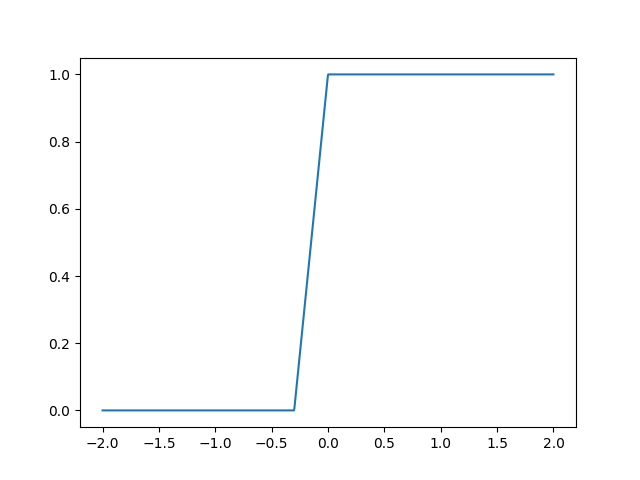
\includegraphics[width=0.7\linewidth]{approx_h.png}
			\caption{$h_{0.3}(x)$}
		\end{center}
	\end{figure}
	
	On a  $\lim_{\epsilon\to0}h_\epsilon = H$ avec $H$ la fonction de Heaviside.
	La fonction $h_\epsilon$ peut être simplement modélisée pour tout $\epsilon>0$ par une structure de réseaux à 4 neurones.
	\subsection{Fonction carré}
	Soit la fonction $g:[0,1]\rightarrow[0, 1], g:x\mapsto min\{2x, 2-2x\}$.
	On a $x^2 = \lim_{x\to\infty} f_n(x)= \lim_{x\to\infty} x - \sum_{s=1}^{n}\dfrac{g_s(x)}{2^{2s}}$\\
	
	On peut modéliser $f_n(x)$ grâce à un réseaux de neurones et donc obtenir des approximations de $x^2$ avec différentes précisions.\\ 
	
	\begin{figure}[H]
		\begin{center}
			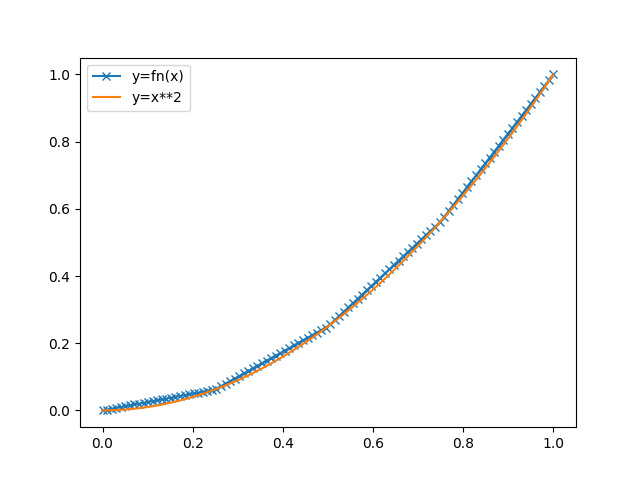
\includegraphics[width=0.7\linewidth]{square_n2.png}
			\caption{$f_2(x)$}
		\end{center}
	\end{figure}
	
	
	\begin{figure}[H]
		\begin{center}
			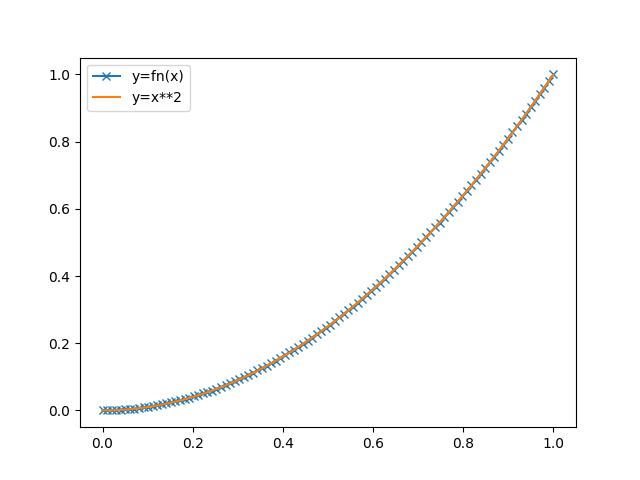
\includegraphics[width=0.7\linewidth]{square_n4.png}
			\caption{$f_4(x)$}
		\end{center}
	\end{figure}
	Pour un n fixé, ce modèle analytique nous donne une erreur maximale égale à $\epsilon_m = 2^{-2m-2}$ ce que l'on retrouve en pratique.
	\begin{center}
		\captionof{table}{Erreurs maximale et moyenne des modèles analytiques}
		\begin{tabular}{ |c||c|c|c|c| } 
			\hline
			n & 1 & 2 & 3 & 4 \\
			\hline
			\hline
			Nombre de neurones & 10 & 20 & 34 & 97\\
			\hline
			Erreur maximale & 0.0624 & 0.0156 & 0.00390 & 0.000976\\
			\hline
			Erreur moyenne & 0.0416 & 0.0103 & 0.00258 & 0.000644\\
			\hline
		\end{tabular}	
	\end{center}
	Le modèle modèlise la fonction $x\mapsto x^2$ seulement sur l'intervalle $[0,1]$
	
	\begin{figure}[H]
		\begin{center}0
			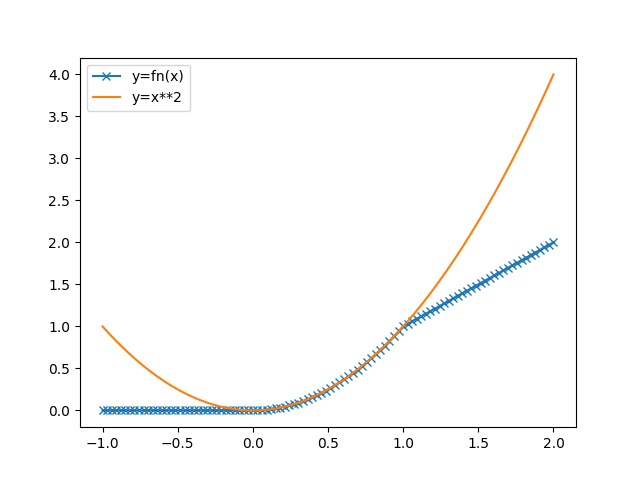
\includegraphics[width=0.7\linewidth]{prolongement_g.png}
			\caption{$f_2(x)$}
		\end{center}
	\end{figure}

	\section{Apprentissage}
	L'idée est de reproduire les résultats des modèles analytiques mais en ajustant les poids par apprentissage.
	J'ai pour cela repris les structures de réseau de neurones des modèles analytiques (même nombre de couches et même nombre de noeuds par couches).\\L'apprentissage est réalisé sur un jeu de 1000 données : les données sources sont 1000 flottants tirés uniformément dans l'intervalle $[0,1]$ et celles cibles sont ces 1000 flottants mis au carré. Ces données sont ensuite séparées en 800 données pour l'entrainement et 200 pour la validation. \\Les tests ont été effectués avec une taille de batch (combien donnée sont examinées avant de mettre à jour les poids) égale à 20 et un nombre d'épochs (nombre de fois que l'on parcours tout l'échantillon) égal à 40. Ces meta-paramètres donnaient en effet un traitement rapide (environ une seconde) pour des résultats relativement consistants comme on le verra plus tard. La méthode d'optimisation choisie est la descente de gradient stochastique. Pour la fonction coût (loss) on utilisera la différence moyenne avec les normes $L_1$ et $L_2$. La mesure d'erreur utilisée sera la norme $L_1$.
	
	On remarque de meilleures performances avec le modèle plus complexe qui comporte plus de couches et plus de poids (détails dans la partie sur les tests), on s'attardera sur le modèle reprenant la structure du modèle analytique pour $n=4$ contenant 7 couches et 52 neurones.
	
	\subsection{Premiers résultats (fonction carré)}
	
	\begin{figure}[H]
		\begin{center}
			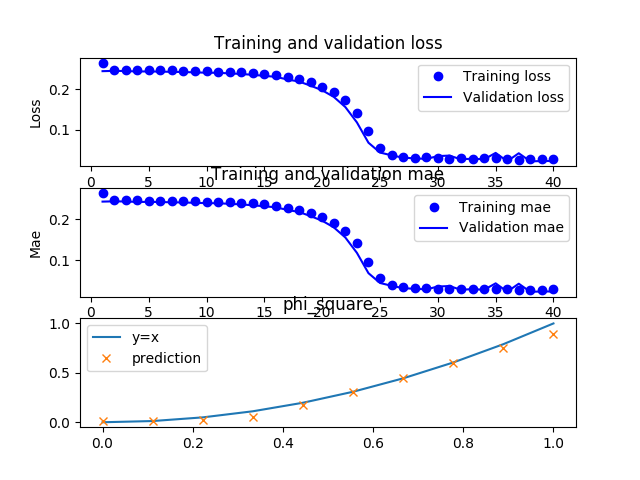
\includegraphics[width=0.7\linewidth]{Figure_1.png}
			\caption{$f_4(x)$ comparé à la fonction $x^2$  avec la fonction coût $L_2$ et la mesure d'erreur exprimées en fonction du nombree d'epochs\\erreur maximale : 0.104, erreur moyenne : 0.028}
		\end{center}
	\end{figure}
	
	On remarque sur cette figure une nette convergence du modèle entre 20 et 25 epochs. La convergence a parfois lieu très rapidement entre 5 et 10 epochs ou parfois progressivement plus tard vers 30 epochs.
	
	Dans environ $10\%$ des cas, on n'a en revanche pas de convergence :
	
	\begin{figure}[H]
		\begin{center}
			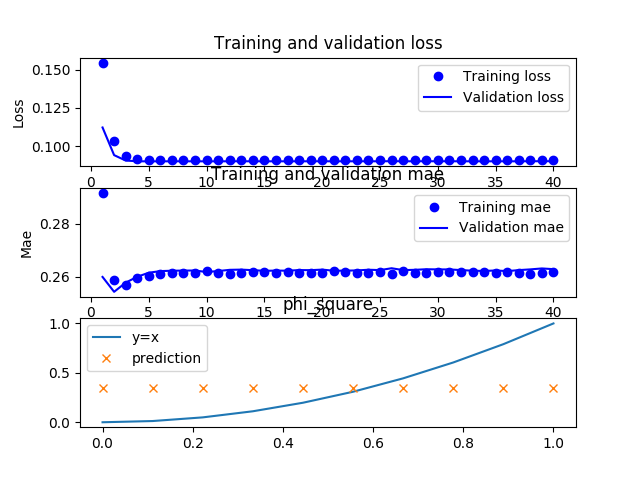
\includegraphics[width=0.7\linewidth]{Figure_4.png}
			\caption{$f_4(x)$ comparée à la fonction $x^2$  avec la fonction coût $L_2$ et la mesure d'erreur exprimées en fonction du nombre d'epochs\\erreur maximale : 0.650, erreur moyenne : 0.278}
		\end{center}
	\end{figure}


	\begin{figure}[H]
		\begin{center}
			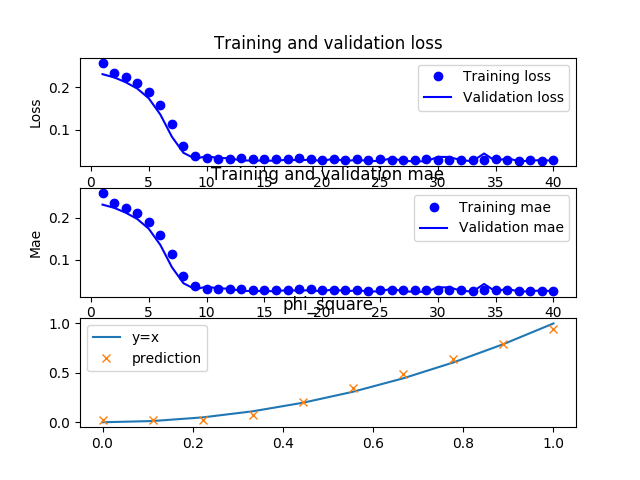
\includegraphics[width=0.7\linewidth]{Figure_6.png}
			\caption{$f_4(x)$ comparée à la fonction $x^2$  avec la fonction coût $L_1$ et la mesure d'erreur exprimées en fonction du nombre d'epochs\\erreur maximale : 0.0548, erreur moyenne : 0.0276}
		\end{center}
	\end{figure}
	La normel $L_1$ donne de meilleurs résultats mais toujours avec des cas de non convergence.

	On remarque aussi qu'en cas de convergence, celle-ci a lieu dans les 40 premiers epochs et qu'après cette convergence le modèle ne s'améliore plus. En particulier peut impporte la durée d'apprentissage on n'arrive pas à retrouver la même précision que dans le modèle analytique analogue. 
	
	\subsection{Prolongement}
	Je me suis ensuite intéressé à savoir quel valeur renverai le modèle pour des points en dehors de l'intervalle sur lequel il a été entrainé et ai tracé la fonction obtenue après l'apprentissage sur l'intervalle $[-1,2]$
	\begin{figure}[H]
		\begin{center}
			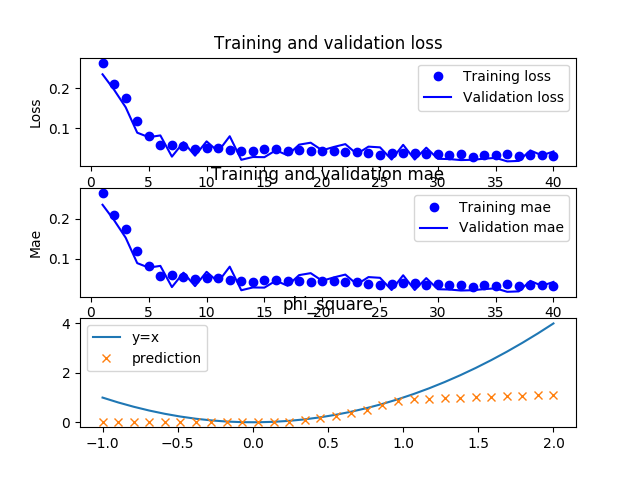
\includegraphics[width=0.7\linewidth]{prolongementx2.png}
			\caption{$f_4(x)$ comparée à la fonction $x^2$  avec la fonction coût $L_2$ et la mesure d'erreur exprimées en fonction du nombre d'epochs}
		\end{center}
	\end{figure}
	On remarque qu'en dehors de l'intervalle d'apprentissage, on obtient des valeurs stationnaires égales à la borne de l'intervalle la plus proche de la valeur testée.
	\subsection{Bruitage}
	J'ai ensuite ajouté sur les échantillons du bruit additif : à chaque échantillon de l'ensemble de donnée est ajouté avec un probabilité $p$ la quantité $\epsilon x$ avec $x$ tiré uniformément sur $[-0.5,0.5]$. 
	 \begin{figure}[H]
	 	\begin{center}
	 		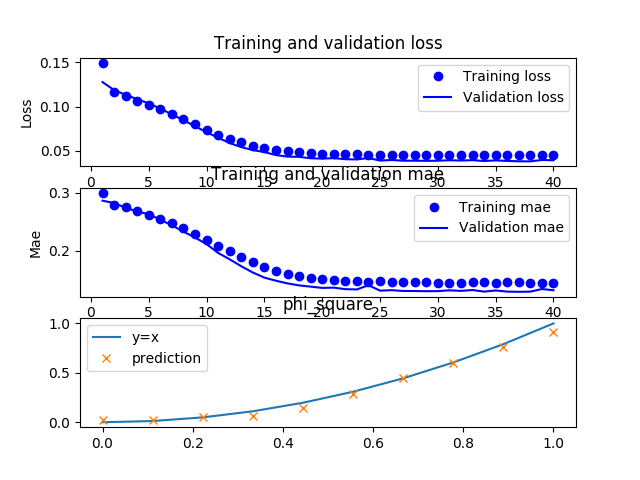
\includegraphics[width=0.7\linewidth]{bruit.png}
	 		\caption{$f_4(x)$ comparée à la fonction $x^2$  avec la fonction coût $L_2$ et la mesure d'erreur exprimées en fonction du nombre d'epochs avec du bruit ajouté avec les paramètres $p=1$ et $\epsilon=1$\\erreur maximale : 0.0843, erreur moyenne : 0.0280}
	 	\end{center}
	 \end{figure}
	On observe obtient après l'apprentissage des résultats très semblable à ceux obtenus sans bruit avec cependant une convergence plus progressive lors de la phase d'apprentissage.
	\subsection{Autres fonctions}
	\subsubsection{Fonction identité}
	Pour la fonction identité, j'ai utilisé un batch de taille 10, cela donnant de meilleurs résultats. En réutilisant le modèle analytique de la fonction identité on obtient de bons résultats.
	\begin{figure}[H]
		\begin{center}
			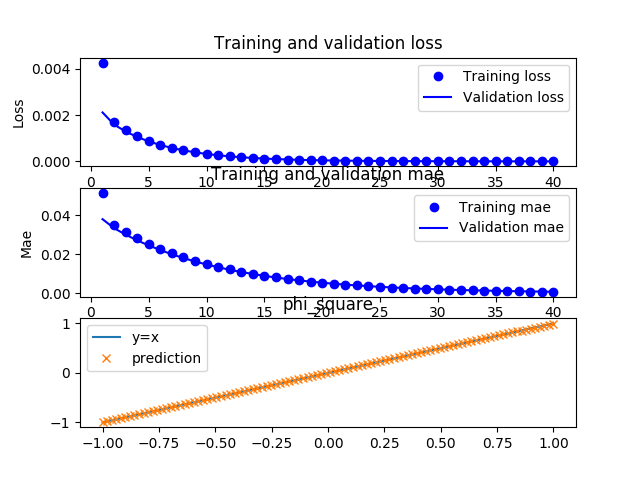
\includegraphics[width=0.7\linewidth]{id_b10_ep40_1.png}
			\caption{Fonction $f$ obtenu par apprentissage comparée à la fonction identité avec la fonction coût $L_2$ et la mesure d'erreur exprimées en fonction du nombre d'epochs}
		\end{center}
	\end{figure}
	Dans le cas particulier précédent on a obtenu après apprentissage des poids très proches des valeurs du modèle analytique et donc un réseau qui fonctionne aussi pour les prolongements.
	
	Dans le cas général on obtient des résultats bon sur l'intervalle d'apprentissage mais des poids très différents de ceux du modèle analytique et donc des résultats non prolongeables.
	

	
	\begin{figure}[H]
		\begin{center}
			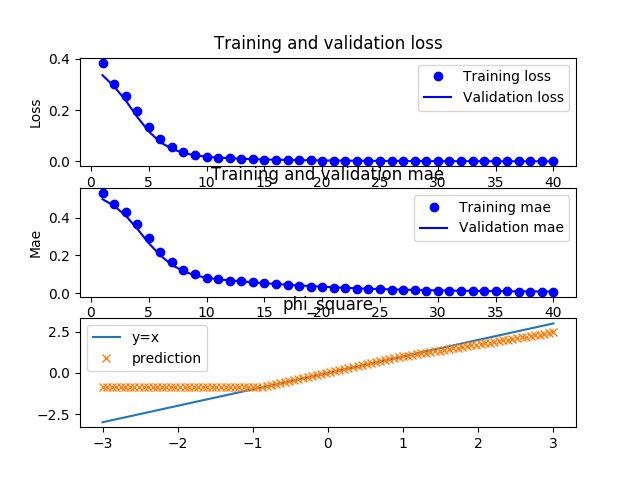
\includegraphics[width=0.7\linewidth]{prolongement_id.png}
			\caption{Fonction $f$ obtenu par apprentissage comparée à la fonction identité avec la fonction coût $L_2$ et la mesure d'erreur exprimées en fonction du nombre d'epochs avec l'apprentissage réalisé seulement sur l'intervalle $[-1,1]$}
		\end{center}
	\end{figure}

	Dans environ $10\%$ des cas on n'a pas de convergence.
	
	\begin{figure}[H]
		\begin{center}
			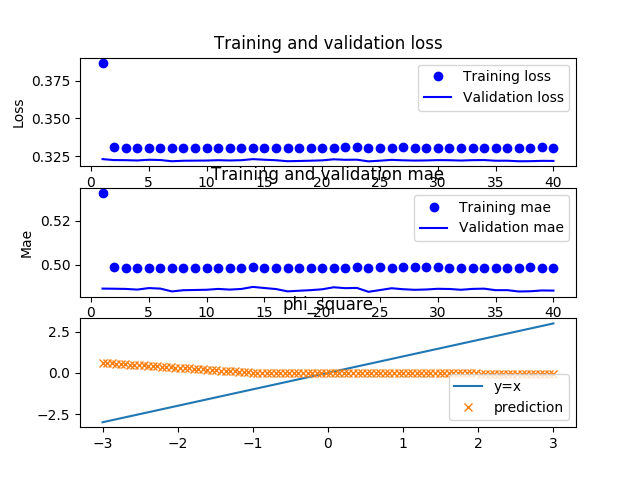
\includegraphics[width=0.7\linewidth]{id_no.png}
			\caption{Fonction $f$ obtenu par apprentissage comparée à la fonction identité avec la fonction coût $L_2$ et la mesure d'erreur exprimées en fonction du nombre d'epochs}
		\end{center}	
	\end{figure}
	
	\subsubsection{Heaviside}
	Pour la fonction de Heaviside, contrairemment à la fonction identité, en utilisant la structure du modèle analytique correspondant on n'obtient jamais de convergence (excepté dans le cas particulier des poids initialisés aux valeurs du modèle analytique où les poids du réseau de neurone restent aux même valeurs lors de l'apprentissage).
	
	\begin{figure}[H]
		\begin{center}
			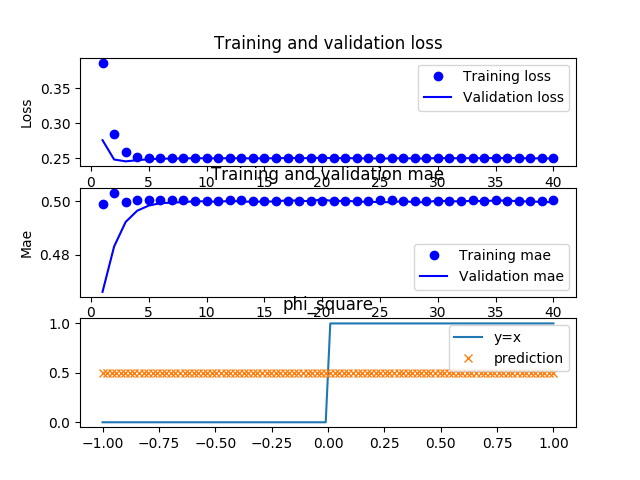
\includegraphics[width=0.7\linewidth]{hvs.png}
			\caption{Fonction $f$ obtenu par apprentissage comparée à la fonction de heaviside avec la fonction coût $L_2$ et la mesure d'erreur exprimées en fonction du nombre d'epochs}
		\end{center}
	\end{figure}
	

	
	\section{Tests généraux}
	\subsection{Fonction carré}
	J'ai considéré que l'on n'avait pas de convergence des poids lors de l'apprentissage quand l'erreur maximale était supérieure à $0.4$ (la fonction prenant ses valeurs dans l'intervalle $[0,1]$).
	\begin{center}
		\captionof{table}{Erreurs moyennes sur 100 répétitions avec SGD}
		\begin{tabular}{ |c||c|c|c| } 
			\hline
			n & 2 & 3 & 4 \\
			\hline
			\hline
			Nombre de cas de convergence & 32 & 66 & 73\\
			\hline
			Erreur maximale & 0.121 & 0.126 & 0.125\\
			\hline
			Erreur moyenne  & 0.0348 & 0.00312 & 0.0276\\
			\hline
			Erreur moyenne intégrale & 0.0348 & 0.0312 & 0.0276 \\
			\hline
		\end{tabular}	
	\end{center}
	On remarque une forte différence de nombre de cas de convergence entre le réseau de structure identique au modèle analytique pour $n=2$ comparé aux deux autres, mais relativement peu de différence quant aux erreurs dans les cas de convergence.
	
	\begin{center}
		\captionof{table}{Erreurs moyennes sur 100 répétitions avec RMSprop}
		\begin{tabular}{ |c||c|c|c| } 
			\hline
			n & 2 & 3 & 4 \\
			\hline
			\hline
			Nombre de cas de convergence & 34 & 75 & 82\\
			\hline
			Erreur maximale & 0.0595 & 0.0333 & 0.0360\\
			\hline
			Erreur moyenne  & 0.0207 & 0.00877 & 0.0111\\
			\hline
			Erreur moyenne intégrale & 0.000700 & 0.000160 & 0.000260 \\
			\hline
		\end{tabular}	
	\end{center}
	On retrouve avec l'optimiseur RMSprop des taux de convergences similaires (légèrement meilleurs) qu'avec la SGD mais de bien meilleurs résultats dans les cas de convergences (erreur maximale 3 fois inférieure pour $n=3$ et $n=4$)\\ \\
	J'ai ensuite effectué les mêmes tests en prenant des structures des réseaux de neurones plus simples consitants en une seule couche de neurones (plus précisement une couche d'opération linéaire, une couche de ReLU et une couche finale d'opération linéiare).
	\begin{center}
		\captionof{table}{Erreurs moyennes sur 100 répétitions avec RMSprop}
		\begin{tabular}{ |c||c|c|c| } 
			\hline
			nombre de neurones & 4 & 10 & 34 \\
			\hline
			\hline
			Nombre de cas de convergence & 81 & 95 & 100\\
			\hline
			Erreur maximale & 0.0673 & 0.0422 & 0.0119\\
			\hline
			Erreur moyenne  & 0.0215 & 0.0123 & 0.00265\\
			\hline
			Erreur moyenne intégrale & 0.000797 & 0.000346 & 0.0000152 \\
			\hline
		\end{tabular}	
	\end{center}
	
	On remarque de bien meilleurs performances qu'avec les réseaux reprenant les structures des modèles analytiques: avec 34 neurones soit le même nombre de neurones que le modèle analytique pour $n=3$ on obtient $100\%$ de cas de convergence avec des erreurs très faibles.
	\subsection{Fonction de Heaviside}
	La fonction de Heaviside n'étant pas continue, le critère de convergence basé sur l'erreur maximale n'est pas adéquat.\\
	En reprenant le modèle constitué d'une unique couche avec l'optimiseur RMSprop, on obtient de bon résultats (avec un taux de convergence élevé) dès 8 neurones, avec cette fois-ci 120 epochs, la convergence étant plus progressive.
	
	\begin{figure}[H]
		\begin{center}
			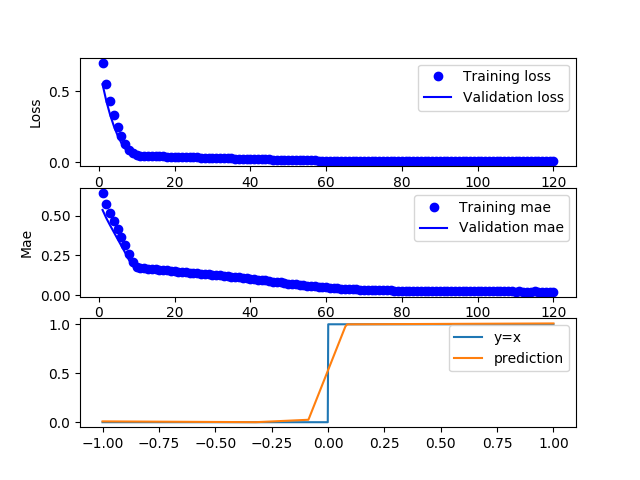
\includegraphics[width=0.7\linewidth]{8.png}
			\caption{10 neurones}
		\end{center}
	\end{figure}
	Augmenter le nombre de neurones avec ce modèle n'amèliore que peu la fonction obtenue, les résulats devenant même moins bon pour des nombres trop élevés.
	\begin{figure}[H]
		\begin{center}
			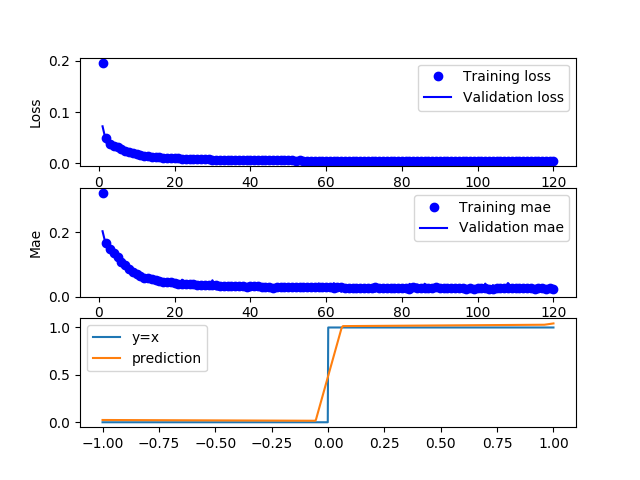
\includegraphics[width=0.7\linewidth]{100.png}
			\caption{100 neurones}
		\end{center}
	\end{figure}
		\begin{figure}[H]
		\begin{center}
			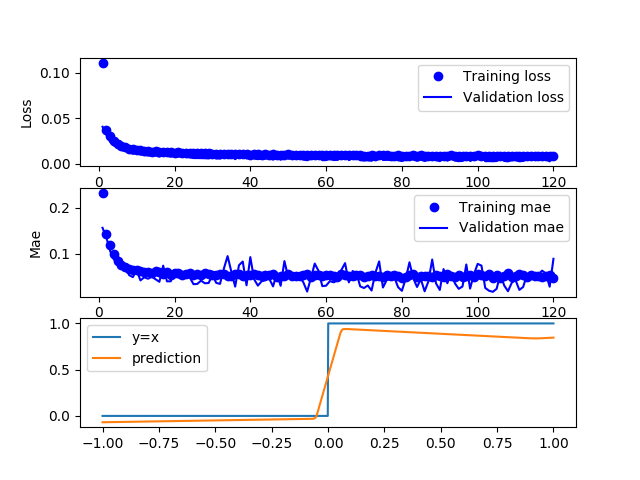
\includegraphics[width=0.7\linewidth]{500.png}
			\caption{500 neurones}
		\end{center}
	\end{figure}
	Contrairement à la fonction carré, le fait d'avoir plusieurs couches est ici bénéfique à la modélisation : avec la structure du modèle analytique de la fonction carré pour $n=4$ contenant 96 neurones on obtient des résultats consistants et meilleurs qu'avec une structure à une seule couche contenant le même nombre de neurones.
	\begin{figure}[H]
	\begin{center}
	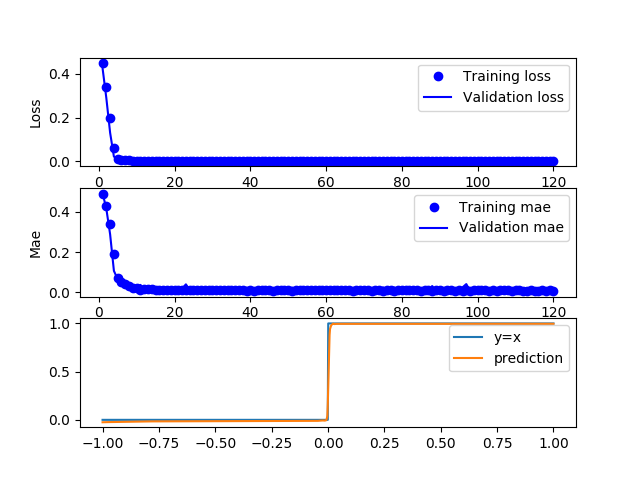
\includegraphics[width=0.7\linewidth]{hvsq.png}
	\caption{Avec la strucutre du modèle analytique de la fonction carré pour $n=4$}
	\end{center}
	\end{figure}
\bibliographystyle{ieeetr}
\bibliography{Bibliographie}
\end{document}